\documentclass{article}

\usepackage{fancyhdr}
\usepackage{extramarks}
\usepackage{amsmath}
\usepackage{amsthm}
\usepackage{amsfonts}
\usepackage{tikz}
\usepackage[plain]{algorithm}
\usepackage{algpseudocode}
\usepackage{enumitem}
\usepackage{forest}
\usepackage[all]{xy}

\usetikzlibrary{automata,positioning}
\graphicspath{{images/}}
%
% Basic Document Settings
%

\topmargin=-0.45in
\evensidemargin=0in
\oddsidemargin=0in
\textwidth=6.5in
\textheight=9.0in
\headsep=0.25in

\linespread{1.1}

\pagestyle{fancy}
\lhead{\hmwkClass}
\chead{\hmwkTitle}
\rhead{\firstxmark}
\lfoot{\lastxmark}
\cfoot{\thepage}

\renewcommand\headrulewidth{0.4pt}
\renewcommand\footrulewidth{0.4pt}

\setlength\parindent{0pt}

%
% Create Problem Sections
%

\newcommand{\enterProblemHeader}[1]{
    \nobreak\extramarks{}{Problema \arabic{#1} continua en la p\'agina siguiente\ldots}\nobreak{}
    \nobreak\extramarks{Problema \arabic{#1} (continuaci\'on)}{Problema \arabic{#1} continua en la p\'agina siguiente\ldots}\nobreak{}
}

\newcommand{\exitProblemHeader}[1]{
    \nobreak\extramarks{Problema \arabic{#1} (continuaci\'on)}{Problema \arabic{#1} continua en la p\'agina siguiente\ldots}\nobreak{}
    \stepcounter{#1}
    \nobreak\extramarks{Problema \arabic{#1}}{}\nobreak{}
}

\setcounter{secnumdepth}{0}
\newcounter{partCounter}
\newcounter{homeworkProblemCounter}
\setcounter{homeworkProblemCounter}{1}
\nobreak\extramarks{Problema \arabic{homeworkProblemCounter}}{}\nobreak{}

%
% Homework Problem Environment
%
% This environment takes an optional argument. When given, it will adjust the
% problem counter. This is useful for when the problems given for your
% assignment aren't sequential. See the last 3 problems of this template for an
% example.
%
\newenvironment{homeworkProblem}[1][-1]{
    \ifnum#1>0
        \setcounter{homeworkProblemCounter}{#1}
    \fi
    \section{Problema \arabic{homeworkProblemCounter}}
    \setcounter{partCounter}{1}
    \enterProblemHeader{homeworkProblemCounter}
}{
    \exitProblemHeader{homeworkProblemCounter}
}

%
% Homework Details
%   - Title
%   - Due date
%   - Class
%   - Section/Time
%   - Instructor
%   - Author
%

\newcommand{\hmwkTitle}{Tarea\ \#1}
\newcommand{\hmwkDueDate}{Octubre 12, 2020}
\newcommand{\hmwkClass}{Matem\'aticas Discretas}
\newcommand{\hmwkClassTime}{}
\newcommand{\hmwkClassInstructor}{Profesora Alma Ar\'evalo Loyola}
\newcommand{\hmwkAuthorName}{\textbf{Sof\'ia Alatorre} \and \textbf{Edson Morales} \and \textbf{ Diego Navarro }}
\newcommand{\hmwkAuthorEmail}{\textbf{sofialatorre313@ciencias.unam.mx} \and \textbf{ edsonmorales_17@ciencias.unam.mx } \and \textbf{ diegonavarro400@ciencias.unam.mx }}

%
% Title Page
%

\title{
    \vspace{2in}
    \textmd{\textbf{\hmwkClass:\ \hmwkTitle}}\\
    \normalsize\vspace{0.1in}\small{Entregar\ el\ \hmwkDueDate\ a las 11:59pm}\\
    \vspace{0.1in}\large{\textit{\hmwkClassInstructor\ \hmwkClassTime}}
    \vspace{3in}
}

\author{\hmwkAuthorName}
\date{ sofialatorre313@ciencias.unam.mx \& edsonmorales\_17@ciencias.unam.mx \& diegonavarro400@ciencias.unam.mx }


\renewcommand{\part}[1]{\textbf{\large Parte \Alph{partCounter}}\stepcounter{partCounter}\\}

%
% Various Helper Commands
%

% Useful for algorithms
\newcommand{\alg}[1]{\textsc{\bfseries \footnotesize #1}}

% For derivatives
\newcommand{\deriv}[1]{\frac{\mathrm{d}}{\mathrm{d}x} (#1)}

% For partial derivatives
\newcommand{\pderiv}[2]{\frac{\partial}{\partial #1} (#2)}

% Integral dx
\newcommand{\dx}{\mathrm{d}x}

% Alias for the Solution section header
\newcommand{\solution}{\textbf{\large Solución}}

% Probability commands: Expectation, Variance, Covariance, Bias
\newcommand{\E}{\mathrm{E}}
\newcommand{\Var}{\mathrm{Var}}
\newcommand{\Cov}{\mathrm{Cov}}
\newcommand{\Bias}{\mathrm{Bias}}

\begin{document}

\maketitle

\pagebreak

\begin{homeworkProblem} [1]
 Nombra tres ramas de la matemática discreta y justifica el porque pertenecen a este grupo.\\
 \\
  \solution\\
  \\
  Una de las ramas sería la Teoría de Conjuntos, ya que en la matemática discreta los conjuntos numerables (incluyendo conjuntos finitos) son su principal objeto de estudio.
  Otro podría ser la Combinatoria, esta que estudia colecciones finitas de objetos que pueden ser combinados u ordenados.
  Y por ultimo estaría la Teoría de Grafos, que por lo regular es considerada parte de la Combinatoria, pero ha evolucionado lo suficiente como para ser considerada una materia por si misma.

\end{homeworkProblem}

\begin{homeworkProblem} [3]
Explica la diferencia entre los conceptos \textit{discreto} y \textit{continuo} en matemáticas.\\
\\
\solution\\
\\
Las matemáticas continuas estudian los conceptos que tienen ámbitos infinitos, tales como la continuidad y el cambio continuo, el sistema de los números reales es el principal de las matemáticas continuas; por otra parte, las matemáticas discretas son la parte encargada del estudio de los conjuntos discretos y sus procesos en matemática son finitos y contables.
\end{homeworkProblem}

\begin{homeworkProblem}
 Menciona la importancia de las matemáticas discretas en las Ciencias de la Computación.\\
 \\
  \solution\\
  \\
  Son importantes ya que esta se encarga de todo aquello que puede ser contado y por supuesto muy bien manejado por la computadora, y en Ciencias de la Computación se podría decir que solo son computables aquellas funciones de conjuntos numerables.

\end{homeworkProblem}

\begin{homeworkProblem} [6]
 ¿Qué es un algoritmo?\\
 \\
 \solution\\
 \\
 Un algoritmo es una serie ordenada de instrucciones, pasos o procesos que llevan a la solución de un determinado problema.

\end{homeworkProblem}

\pagebreak

\begin{homeworkProblem}
¿Qué es un lenguaje formal?\\
 \\
 \solution\\
 \\
 un lenguaje formal es un lenguaje cuyos símbolos primitivos y reglas para unir esos símbolos están formalmente especificados.Al conjunto de los símbolos primitivos se lo llama el alfabeto (o vocabulario) del lenguaje, y al conjunto de las reglas se lo llama la gramática formal (o sintaxis). A una cadena de símbolos formada de acuerdo a la gramática se la llama una fórmula bien formada (o palabra) del lenguaje. Estrictamente hablando, un lenguaje formal es idéntico al conjunto de todas sus fórmulas bien formadas.

\end{homeworkProblem}

\begin{homeworkProblem}
¿Cuáles son las diferencias entre lenguaje formal y \textit{lenguaje natural}?\\
\\
\solution\\
\\
El lenguaje natural es el que ha surgido de manera natural a través de la historia, ha experimentado cambios con el tiempo y sirve para la comunicación entre animales, entre ellos incluido el propio ser humano y sus distintos idiomas. En cambio, el lenguaje formal es artificial; es decir, inventado para uno o varios propósitos definidos y está compuesto por reglas precisas y fijas.
\end{homeworkProblem}

\begin{homeworkProblem}
¿Qué es una \textit{gramática formal} Menciona su importancia y sus aplicaciones en las Ciencias de la Computación.\\
\\
\solution\\
\\
Una gramática formal es un conjunto de reglas relativas a la sintaxis de un lenguaje; su importancia radica en construir expresiones para un lenguaje e identificar o reconocer expresiones de ese lenguaje para darle sentido y forma al alfabeto, los símbolos terminales, el símbolo inicial y sus reglas de producción.
Sus aplicaciones en las Ciencias de la Computación son para que haya una comunicación estructurada y bien definida entre la computadora y el programador.
\end{homeworkProblem}

\begin{homeworkProblem} [10]
¿Cómo se define una \textit{gramática formal}?\\
\\
\solution\\
\\
Una gramática formal es una estructura lógico-matemática con un conjunto de reglas de formación que definen las cadenas de caracteres admisibles en un determinado lenguaje formal o lenguaje natural.
\end{homeworkProblem}

\begin{homeworkProblem}
 En a lo más 15 lineas, escribe una pequeña biografía de Kurt Gödel incluyendo sus aportaciones más importantes. Inserta una imagen de él al derecho del texto, de tal manera que la imagen ocupe la mayor cantidad de líneas posibles. Consulta tres fuentes distintas y cítalas.\\
 \\
  \solution\\
  \\
  Kurt Gödel. Fue un lógico, matemático, y filósofo austriaco. Reconocido como uno de los más importantes lógicos de todos los tiempos. El trabajo de Gödel ha tenido un impacto inmenso en el pensamiento científico y filosófico del siglo XX.\\

  Gödel, al igual que otros pensadores, intentó emplear la lógica y la teoría de conjuntos para comprender los fundamentos de la matemática. A él se le deben los teoremas de la incompletitud, publicados en 1931. Para demostrar uno de sus teoremas desarrolló una técnica denominada como numeración de Gödel, el cual codifica expresiones formales como números naturales.\\

  También demostró que la hipótesis del continuo no puede refutarse desde los axiomas aceptados de la teoría de conjuntos, si dichos axiomas son consistentes. Realizó importantes contribuciones a la teoría de la demostración al esclarecer las conexiones entre la lógica clásica, la lógica intuicionista y la lógica modal.\\

  En 1933 Gödel viajó por primera vez a los Estados Unidos donde conoció a Albert Einstein, con quien estrechó lazos de amistad. Presentó una conferencia en la reunión anual de la Sociedad Americana de Matemáticas. En el transcurso de ese año Gödel también desarrolló ideas sobre la computabilidad y la función recursiva al punto que presentó una conferencia sobre dichas funciones y sobre el concepto de verdad. Posteriormente, este trabajo se desarrolló en la teoría de los números, empleando la numeración de Gödel.\\

  En 1951 Gödel fue reconocido (junto a Julian Schwinger) con el primer Premio Albert Einstein, y también se le entregó la National Medal of Science en 1974.\\
  \begin{figure}[h]
      \center
      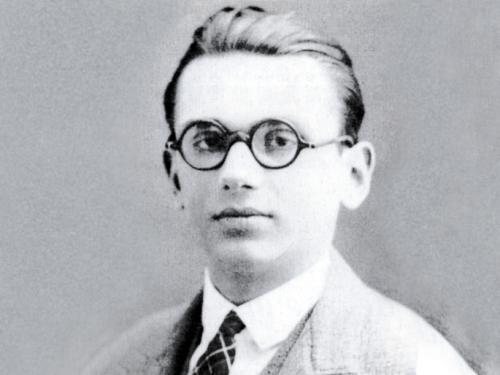
\includegraphics[scale=0.5]{Godel}
      \caption{Kurt Gödel}
      \label{fig:my_label}
  \end{figure}

  Fuentes Consultadas:\\
  https://www.ecured.cu/Kurt\_Gödel\\
  https://es.wikipedia.org/wiki/Kurt\_Gödel\\
  https://www.bbc.com/mundo/noticias-43568588\\

  \end{homeworkProblem}

  \begin{homeworkProblem} [13]
  ¿Es mejor tener muchas o pocas reglas para un lenguaje? Justifica tu respuesta.\\
  \\
  \solution\\
  \\
  Yo pienso que un lenguaje al tener demasiadas reglas lo hace un poco más complejo, ya que en el caso de estar programando, el usuario se vería sometido a utilizar muchas expresiones o por decirlo así, tardaría demasiado en enviar una instrucción. En cambio uno con pocas reglas lo hace mucho más compacto y dinamico.\\

  \end{homeworkProblem}

\begin{homeworkProblem}
  ¿Es posible que una misma cadena pertenezca a más de un lenguaje?
  Argumenta tu respuesta. Si la respuesta es afirmativa, proporciona un ejemplo.\\
  \\
  \solution\\
  \\
  Si.\\
  \\
  \textbf{Ejemplo:}\\
  \\
  Sea la gramática de un lenguaje $A$, dada por $G = \{ \Sigma, T, S,P \}$
  donde $\Sigma = {a,b,c,\dots, z} $, $T = \Sigma$ y las producciones
  cualquier combinación de elementos del alfabeto,
  y la gramática del lenguaje $B$,todo lo mismo que la $A$, menos las
  producciones que son dadas por todas las palabras que sean del español. Podemos
  decir que nuestro diccionario es el siguiente conjunto $D = \{"perro"\}$. Vemos
  que $perro$, pertenece a estos dos lenguajes. Se pueden agregar muchas
  más palabras al diccionario, y se puede ver que siempre se cumple que el segundo
  lenguaje esta contenido en el primero.\\
\end{homeworkProblem}

\pagebreak

\begin{homeworkProblem}
  Utilizando la gramática para el lenguaje de las cadenas de paréntesis
  balanceados decide cuales de las siguientes cadenas están bien construidas
  utilizando sus arboles de derivación:\\
  \begin{enumerate}[label=\Alph*]
    \item{(()()))}
    \item{(()())(())}
    \item{(()()())(())}
    \item{(((()))))()}
  \end{enumerate}

  \solution\\
  \\
  \part\\
  \\
  Vemos a \textsc{(()()))}, ahora según la gramática de los paréntesis balanceados,
  tenemos que tener siempre la misma cantidad de paréntesis derechos, que de izquierdos.\\
  \\
  Contamos que hay 3 paréntesis derechos, mientras que hay 4 paréntesis derechos. Por esto
  podemos decir que no pertenece a esta gramática.\\
  \\
  \part\\
  \\
  Veamos que pasa con \textsc{(()())(())}, podemos ver por su árbol de generación que si es parte
  de la gramática:\\
  \\
  \begin{center}
    \begin{forest}
      [S
        [(E)
         [(E)
           [()]
           [$\epsilon$]
         ]
         [E
           [(E)
            [()]
            [$\epsilon$]
           ]
         ]
        ]
        [E
          [(E)
            [(E)
              [()]
              [$\epsilon$]
            ]
          ]
          [E
            [$\epsilon$]
          ]
        ]
      ]
    \end{forest}
  \end{center}

  Esto siendo el árbol de generación de nuestra cadena a probar. Podemos ver que
  si es parte de esta gramática.\\
  \\
  \part\\
  \\
  Vemos ahora que pasa con \textsc{(()()())(())}, podemos ver el árbol de generación,
  con esto podemos estar seguro que pertenece. Y se ve de la siguiente manera:\\

  \begin{center}
    \begin{forest}
      [S
        [(E)
         [(E)
           [()]
           [$\epsilon$]
         ]
         [E
           [(E)
             [()]
             [$\epsilon$]
           ]
           [E
            [(E)
               [()]
               [$\epsilon$]
            ]
            [E
               [$\epsilon$]
            ]
           ]
         ]
        ]
        [E
          [(E)
            [(E)
              [()]
              [$\epsilon$]
            ]
          ]
          [E
            [$\epsilon$]
          ]
        ]
      ]
    \end{forest}
  \end{center}

  Como podemos ver, podemos llegar a la cadena deseada, usando las reglas
  gramaticales. Gracias a esto podemos concluir que por tanto, la cadena
  pertenece a la gramática.\\
  \\
  \part\\
  \\
  Podemos ver que para este problema el numero de paréntesis que abren y que cierran
  no es el mismo, por eso podemos ver que no podría existir árbol de generación.
  En este caso vemos que el \textsc{(((()))))()} cuenta con 5 paréntesis izquierdos,
  pero en el caso de los paréntesis derechos cuenta con 6, así haciéndolo un caso
  imposible de generar por la gramática dada.
\end{homeworkProblem}

\begin{homeworkProblem}[29]
  Investiga sobre las expresiones regulares y responde lo siguiente: ¿qué son?, ¿para qué se utilizan? y ¿cuál es su relación con los lenguajes formales?\\
  \\
  \solution\\
  \\
  Una expresión regular, también conocida como regex, es una secuencia de caracteres que conforma un patrón de búsqueda. Se utilizan principalmente para la búsqueda de patrones de cadenas de caracteres u operaciones de sustituciones.\\

  Se podría decir que una relación con un lenguaje formal, es que una expresión regular es una forma de representar los lenguajes regulares (finitos o infinitos) y se construye utilizando caracteres del alfabeto sobre el cual se define el lenguaje.


  \end{homeworkProblem}


\begin{homeworkProblem}[30]
  ¿Puede existir más de una gramática para un mismo lenguaje? Justifica tu respuesta plenamente.
  En dado caso de que la respuesta sea \textbf{SI} selecciona alguna de las gramáticas con las que hemos
  trabajado a lo largo de la tarea y brinda un ejemplo de esto.\\
  \\
  \solution \\
  \\
  Puede existir más de una gramática para un mismo lenguaje. Así propongo las siguientes gramáticas
  que nos dan el mismo lenguaje. Tomamos por ejemplo el caso del ejercicio 17 de esta tarea donde
  se propone una gramática:\\
  \\
  Considerando la siguiente $G = {\Sigma, T, S, P}$ donde $\Sigma = {a, b, c, S}$ es el alfabeto, $T = {a, b, c}$ es
  el conjunto de símbolos terminales, $S$ es el símbolo inicial y $P$ son las siguientes producciones:
  $S \rightarrow abS, S \rightarrow bcS, S \rightarrow bbS, S \rightarrow a, S \rightarrow cb$.\\
  \\
  Esta siendo nuestra gramática $A$, vemos que si proponemos una gramática diferente que nos de el mismo
  lenguaje, estaríamos teniendo un contraejemplo de que para todo lenguaje $L \exists! G$.\\
  \\
  La gramática que se propone es la siguiente:\\
  \\
  Considerando la siguiente $G_1 = {\Sigma_1, T_1, S_1, P_1}$ donde $\Sigma_1 = {a, b, c, S}$ es el alfabeto, $T_1 = {a, b, c}$ es
  el conjunto de símbolos terminales, $S_1$ es el símbolo inicial y $P_1$ son las siguientes producciones:
  $S \rightarrow abS, S \rightarrow bES, S \rightarrow bcS, S \rightarrow a, S \rightarrow cb, E \rightarrow b $.\\
  \\
  Podemos ver que esta gramática genera lo mismo, ya que E, solo regresa como un resultado a $"b"$, y solo se usa en
  el lugar donde podríamos poner a $"b"$, entonces, bien se puede hacer la simplificación de esta a la anterior
  sin pedir muchas cosas de nuestras reglas. Solamente se hace una sustitución en un lugar.\\
  \\
  Por esto entonces podemos concluir que si es posible para algún lenguaje que existan 2 o más gramáticas
  que lo generen.
\end{homeworkProblem}

\begin{homeworkProblem} [33]
Investiga qué es una \textit{gramática libre de contexto} y menciona cuál de las gramáticas con las que hemos trabajado a lo lardo de la tarea o ayudantías cumple con serlo.\\
\\
\solution\\
\\
Una gramática de libre contexto es una gramática formal en la que cada regla de producción es de la forma: \xymatrix{*+<2em>{V} \ar[r] & w}\\
Donde V es un \textbf{símbolo no terminal} y w es una cadena de terminales y/o no terminales. El no terminal V siempre puede ser sustituido por w sin tener en cuenta el contexto en el que ocurra.
La notación más frecuentemente utilizada para expresar gramáticas de libre contexto es la Backus-Naur.\\
\\
\textbf{Ejemplos}\\
\\
Dado un lenguaje, construir la gramática:
\begin{enumerate}
\item Cadenas de bits {o,1} que empiezan con 0 y terminan con 1.\\
$T = \{ 0, 1 \}$\\
$S ::= OE1$\\
$E ::= 0 | 1 | \epsilon | EE$\\
\\
\item Cadenas de puros ceros con longitud impar.\\
$T = \{ 0, 1 \}$\\
$S ::= 0 | OOS$\\
\\
\item Cadenas de ceros con longitud par.\\
$T = \{ 0, 1 \}$\\
$S ::= \epsilon | 00S $\\
\\
\item Cadenas palíndromas de bits.\\
$T = \{ 0, 1 \}$\\
$S ::= 0S0 | 1S1 | 00 | 11 | 0 | 1$\\
\end{enumerate}
\end{homeworkProblem}


\begin{homeworkProblem}[36]
  \textbf{Cierto o falso} (justifica brevemente): Existe un algoritmo tal que para cualquier lenguaje
  determine el conjunto de expresiones mínimas que genere dicho lenguaje.\\
  \\
  \solution\\
  \\
  \textbf{Falso}. Podemos ver que no siempre que queramos tener un lenguaje podemos
  saber que la gramática mínima que lo genere, ya que supongamos que existe un lenguaje
  A, que es el lenguaje de las expresiones gramáticas, y supongamos que es el mínimo,
  con el cual podemos generar a todas las reglas gramaticales que generan a todos
  los lenguajes posibles. Ya que podríamos generar una infinidad de lenguajes nuevos,
  lo único que podríamos decir es que si existe un lenguaje que pueda generarse con
  una cantidad finita de reglas, si las reglas son recursivas, y si las referencias
  no son cíclicas, podemos decir que estamos en un camino aceptable con menor cantidad
  de reglas.\\
  \\
  Ahora tratando de ser más formal, podemos decir que El lenguaje de los lenguajes formales
  es un lenguaje formal. Como la definición de que es lo que es valido dentro de este lenguaje
  esta dada en ese lenguaje. Esto entonces dando como resultado una teoría que se define con
  la definición, entonces encontrar una demostración, de que es valido o no un mínimo de
  reglas,  ya que al momento de definir estas, posiblemente no estamos contando todo lo que se tenga.\\
\end{homeworkProblem}

\section{Bibliografía}
\begin{itemize}
\item https://es.wikipedia.org/wiki/Gram%C3%A1tica_libre_de_contexto#Ejemplo_1
\item https://es.wikipedia.org/wiki/Gram%C3%A1tica_libre_de_contexto
\item http://estructurasmatematicas.blogspot.com/2009/04/matematica-discreta.html
\end{itemize}


\end{document}
